\documentclass[handout]{beamer}
%%%%%%%%%%%%%%%%%%%%%%%%%% DO NOT MODIFY %%%%%%%%%%%%%%%%%%%%%%%%%
%% preamble
\usetheme{Madrid}
\mode<presentation>
\usepackage[spanish]{babel}
\usepackage[utf8]{inputenc}
\usepackage{lmodern}
\usepackage{hyperref}
\usepackage{listings}
\usepackage[T1]{fontenc}

\defbeamertemplate*{footline}{shadow theme}{%
  \leavevmode%
  \hbox{\begin{beamercolorbox}[wd=.5\paperwidth,ht=2ex,dp=1ex,leftskip=.3cm plus1fil,rightskip=.3cm]{author in head/foot}%
      \usebeamerfont{author in head/foot}\hfill\insertshortauthor
  \end{beamercolorbox}%

  \begin{beamercolorbox}[wd=.5\paperwidth,ht=2ex,dp=1ex,leftskip=.3cm,rightskip=.3cm plus1fil]{title in head/foot}%
      \usebeamerfont{title in head/foot}\insertshorttitle\hfill%
  \insertframenumber\,/\,\inserttotalframenumber
  \end{beamercolorbox}}%
  \vskip0pt%
}

\AtBeginSection[]{
  \begin{frame}[allowframebreaks]{Contenido}
  \small{\tableofcontents[currentsection]}
  \end{frame}
}

\AtBeginSubsection[]{
  \begin{frame}[allowframebreaks]{Contenido}
    \small{\tableofcontents[currentsubsection]}
  \end{frame}
}
\beamertemplatenavigationsymbolsempty 
\usefonttheme[onlymath]{serif}

\lstdefinestyle{customHTML}{
  belowcaptionskip=1\baselineskip,
  breaklines=true,
  frame=L,
  xleftmargin=\parindent,
  language=HTML,
  showstringspaces=false,
  basicstyle=\footnotesize\ttfamily,
  keywordstyle=\bfseries\color{blue},
  commentstyle=\itshape\color{gray},
  identifierstyle=\color{black},
  stringstyle=\color{orange},
}
\lstset{escapechar=@,style=customHTML}

%%%%%%%%%%%%%%%%%%%%%%%%% END DO NOT MODIFY %%%%%%%%%%%%%%%%%%%%

\title{Introducción a la Programación}
\subtitle{Variables}
\author{Edwin Salvador}
\date{14 de junio de 2016}
\begin{document}
  \begin{frame}
    \titlepage
    \centerline{Clase 9}
  \end{frame}
  
  \AtBeginSection[]{
    \begin{frame}[allowframebreaks]{Contenido}
      \tableofcontents[currentsection]
    \end{frame}
  }

\section{Variables} % (fold)
\label{sec:variables}
\begin{frame}[t]{Variables}
    \begin{itemize}
      \item Representan un espacio en memoria
      \item Almacenan datos temporalmente
      \item Se componen de un tipo de datos y un nombre (comienza con una letra y no tiene espacios, signos de puntuación u operadores)
      \item Pueden cambiar su valor pero siempre debe ser del mismo tipo.
    \end{itemize}
\end{frame}

\begin{frame}[t]\frametitle{Ejemplos Identificadores}
    \begin{itemize}
      \item Ejemplo de identificadores válidos (\textbf{convenciones}):
        \begin{itemize}
          \item fecha
          \item fec
          \item fechaNacimiento
          \item fechaNac
          \item fec1
          \item fec2
          \item iFechaNac
        \end{itemize}
      \item \textbf{No válidos}
      \begin{itemize}
        \item 2fecha (no puede comenzar con un número)
        \item -fecha (no puede comenzar con un signo ``menos'')
        \item fecha nacimiento (no puede tener espacios en blanco)
        \item fecha-nacimiento (no puede tener el signo ``menos'')
        \item fecha+nacimiento (no puede tener el signo ``más'') 
      \end{itemize} 
    \end{itemize}
\end{frame}
% section variables (end)

\section{\texttt{printf}} % (fold)
\label{sec:printf}
\begin{frame}[t]\frametitle{\texttt{printf}}
    \begin{itemize}
      \item Permite mostrar datos en la consola ya sea texto fijo o variables.
      \item Permite el uso de ``máscaras'', se le debe pasar tantos datos como máscaras.
      \item Ejemplo 
    \end{itemize}
\end{frame}
% section printf (end)

\section{\texttt{scanf}} % (fold)
\label{sec:scanf}
\begin{frame}[t]\frametitle{\texttt{scanf}}
    \begin{itemize}
      \item Permite leer datos del teclado y los asigna a una variable que le pasemos como argumento.
      \item También utiliza máscaras
      \item Se le debe pasar la referencia o dirección de memoria de la variable que donde se desea almacenar el valor. Esto lo obtenemos anteponiendo el operador \& (léase “operador ampersand”).
      \item Ejemplo 
    \end{itemize}
\end{frame}
% section scanf (end)

\section{Constantes} % (fold)
\label{sec:constantes}
\begin{frame}[t]\frametitle{Constantes}
    \begin{itemize}
      \item En algunos problemas pueden existir valores que no cambian.
      \item Ejemplo: PI = 3.141592654 y E = 2.718281828
      \item \texttt{\#define NUMERO\_PI 3.1415169254}
      \item \texttt{\#define NUMERO\_E 2.718281828}
      \item El modificador \texttt{const} evitará que el valor de una variable cambie 
      \item \texttt{const int temperaturaMaxima = 45;}
      \item Las constantes deben ser escritas completamente en mayúsculas

    \end{itemize}
\end{frame}
% section constantes (end)

\section{Ejemplos} % (fold)
\label{sec:ejemplos}
\begin{frame}[t]\frametitle{Ejemplos: suma de dos números}
    \begin{figure}[tb]
      \centering
      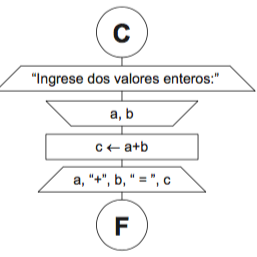
\includegraphics[scale=.7]{./img/suma2}
    \end{figure}
\end{frame}


\begin{frame}[t]\frametitle{Ejemplos: división de dos números}
    \begin{figure}[tb]
      \centering
      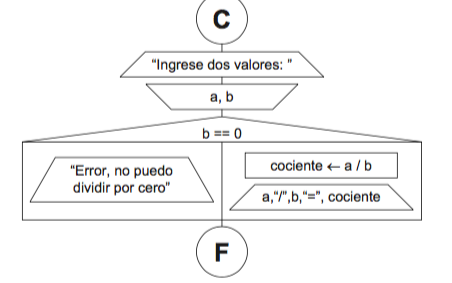
\includegraphics[scale=.7]{./img/div2}
    \end{figure}
\end{frame}

% section ejemplos (end)

\section{Conversión de tipos de datos (type casting)} % (fold)
\label{sec:conversion_de_tipos_de_datos}
\begin{frame}[t]\frametitle{Conversión de tipos de datos (type casting)}
  \begin{itemize}
    \item El operador \texttt{/} convierte el resultado al mayor tipo de datos de sus operandos.
    \item Si dividimos dos \texttt{int} el resultado siempre será \texttt{int}.
    \item \texttt{cociente = a/b;}
    \item Si el tipo de datos de \texttt{cociente} es \texttt{double} debemos convertir uno de los operandos a ese tipo de datos.
    \item \texttt{cociente = (double)a/b;}
    \item El mayor tipo de datos entre \texttt{int} y \texttt{double} es \texttt{double} por lo tanto el resultado será convertido a \texttt{double}
    \item Escribir el programa con el casting y sin el casting para comparar resultados.
  \end{itemize}
  
\end{frame}
% section conversión_de_tipos_de_datos_ (end)

\section{El operador \% (``módulo'' o ``resto'')} % (fold)
\label{sec:el_operador__modulo_o_resto_}
\begin{frame}[t]\frametitle{El operador \% (``módulo'' o ``resto'')}
    
\texttt{int a = 5;}\\
\texttt{int b = 3;} \\
\texttt{int r = a \% b;}


\end{frame}

\begin{frame}[t]\frametitle{Ejemplo módulo}
    \begin{itemize}
      \item Verificar si el número que ingresa el usuario por teclado es par o impar       
    \end{itemize}

    \begin{figure}[tb]
      \centering
      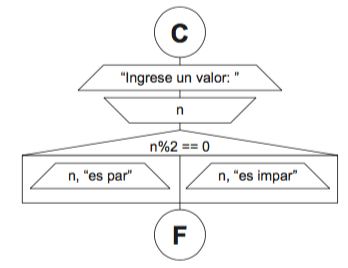
\includegraphics[scale=.7]{./img/mod}
    \end{figure}

\end{frame}
% section el_operador__modulo_o_resto_ (end)

\section{Operadores Relacionales} % (fold)
\label{sec:operadores_relacionales}
\begin{frame}[t]\frametitle{Operadores Relacionales}
    
\begin{figure}[tb]
  \centering
  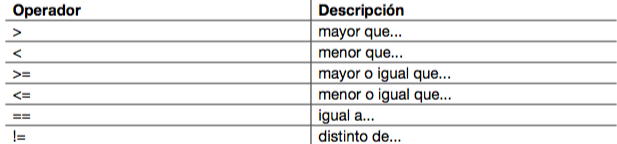
\includegraphics[scale=.6]{./img/oprela}
\end{figure}

\end{frame}
% section operadores_relacionales (end)

\section{Expresiones lógicas} % (fold)
\label{sec:exmpresiones_logicas}
\begin{frame}[t]\frametitle{Expresiones lógicas}
        
\begin{itemize}
  \item Pueden ser verdaderas o falsas
  \item 2 < 5
  \item 2 + 1 = 4
  \item Hola = Hola
\end{itemize}
\end{frame}

\begin{frame}[t]\frametitle{Operadores lógicos}
    
\begin{figure}[tb]
  \centering
  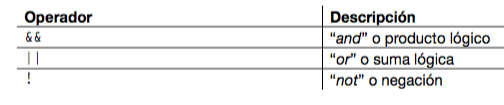
\includegraphics[scale=.7]{./img/oplog}
\end{figure}

\end{frame}

\begin{frame}[t]\frametitle{Operadores AND (\&\&)}
    
\begin{figure}[tb]
  \centering
  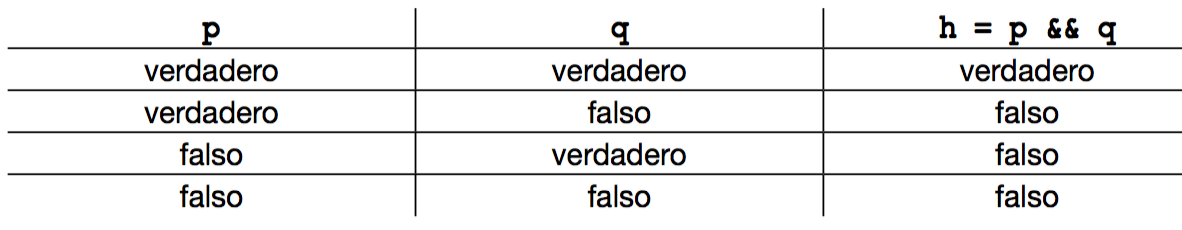
\includegraphics[scale=.5]{./img/oplog1}
\end{figure}

\end{frame}

\begin{frame}[t]\frametitle{Operadores OR (||)}
    
\begin{figure}[tb]
  \centering
  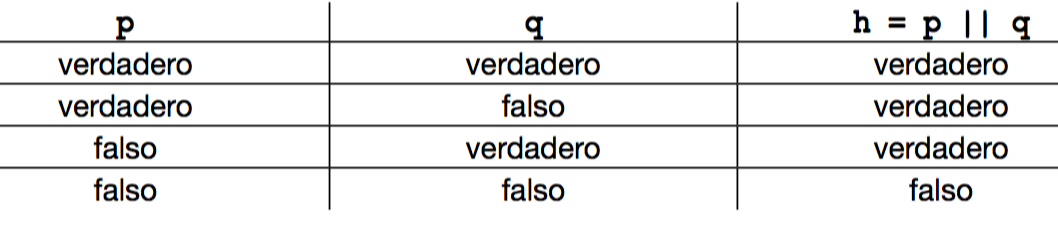
\includegraphics[scale=.5]{./img/oplogOR}
\end{figure}

\end{frame}

\begin{frame}[t]\frametitle{Operadores NOT (!)}
    
\begin{figure}[tb]
  \centering
  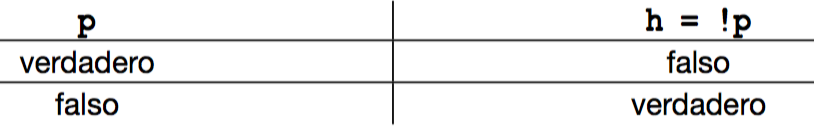
\includegraphics[scale=.5]{./img/oplogNOT}
\end{figure}

\end{frame}
% section expresiones_lógicas (end)

\section{Estructuras de control} % (fold)
\label{sec:estructuras_de_control}
\subsection{Estructura de Decisión} % (fold)
\label{sub:estructura_de_decision}

\begin{frame}[t]\frametitle{Estructura de decisión}
    
Ejemplo
\begin{itemize}
  \item Leer dos valores numéricos enteros e indicar cuál es el mayor y cuál es el menor. Considerar que ambos valores son diferentes.
  \begin{figure}[tb]
     \centering
     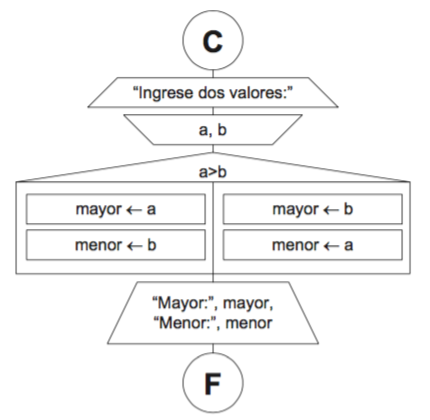
\includegraphics[scale=.7]{./img/if}
   \end{figure} 
\end{itemize}


\end{frame}

\begin{frame}[t]\frametitle{Estructuras de decisión anidadas}
    
Cuando una estructura de decisión está dentro de otra. Ejemplo:
\begin{itemize}
  \item Leer tres valores numéricos enteros, indicar cuál es el mayor, cuál es el del medio y cuál, el menor. Considerar que los tres valores serán diferentes.
  \begin{figure}[tb]
    \centering
    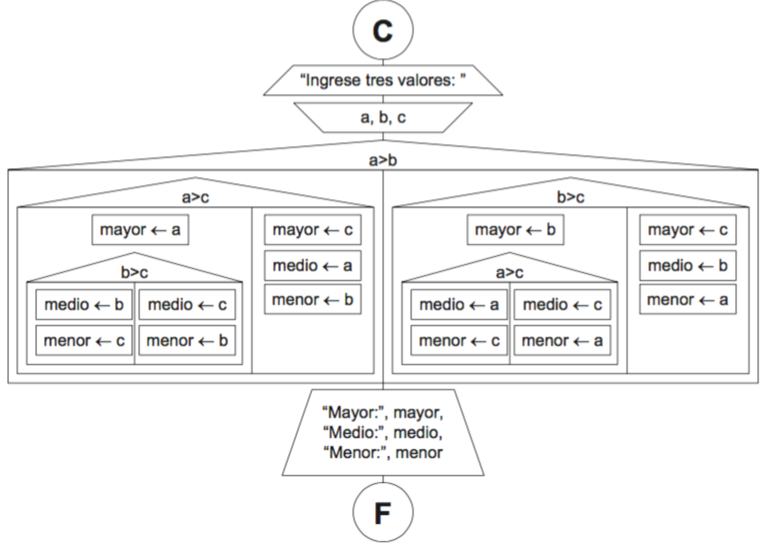
\includegraphics[scale=.6]{./img/ifani}
  \end{figure}
 
\end{itemize}


\end{frame}

\begin{frame}[t]\frametitle{Una mejor solución al ejercicio anterior}
    Es mejor evitar anidar muchos \texttt{if}, para eso podemos utilizar los operadores lógicos y también el \textbf{if en una línea}
\begin{figure}[tb]
  \centering
  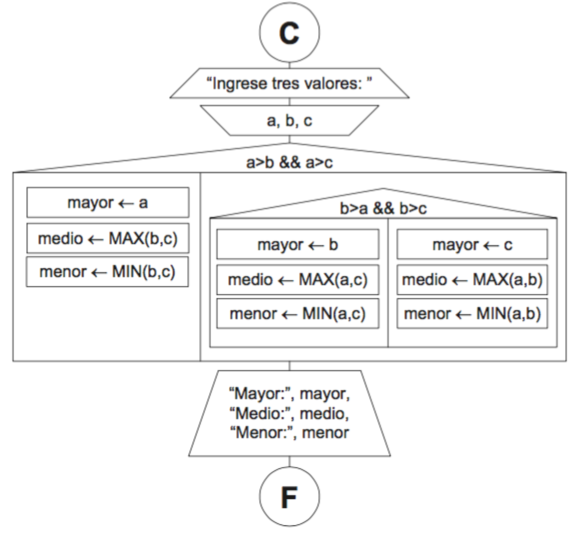
\includegraphics[scale=.6]{./img/ifani2}
\end{figure}

\end{frame}


% subsection estructura_de_decisión (end)
% section estructuras_de_control (end)
\end{document}
